\documentclass{article}
\usepackage{pgfplots}
\pgfplotsset{compat=1.18}
\begin{document}
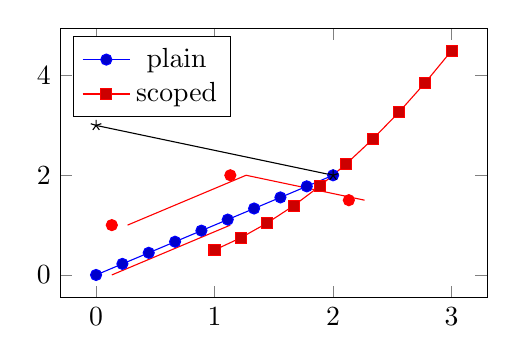
\begin{tikzpicture}[thick, every path/.append style={line cap=butt}]
  \begin{axis}[width=7cm, height=5cm, domain=0:2, samples=10, legend pos=north west]
    \addplot {x};
    \addlegendentry{plain}
    \begin{scope}[red, /pgfplots/domain=1:3]
      \addplot {x^2/2};
      \addlegendentry{scoped}
      \begin{scope}[xshift=2mm]
        \addplot[mark=*] coordinates {(0,1) (1,2) (2,1.5)};
        \draw (axis cs:0,0) -- (axis cs:1,1);
      \end{scope}
    \end{scope}
    \addplot coordinates {(0,3) (2,2)};
  \end{axis}
\end{tikzpicture}
\end{document}
